\documentclass[12pt,a4paper]{article}
\usepackage{amsmath}
\usepackage{tikz}
\usetikzlibrary{arrows.meta}

\begin{document}

An example for Lemma~\ref{common boundary points lemma}: $K$ (black), $-K$ (dashed), $\underline{M}_{0}(K,-K)$ (orange), $\overline{M}_{1}(K,-K)$ (blue), $\overline{M}_{3}(K,-K)$ (red), $\overline{M}_{\infty}(K,-K)$ (dashdotted).

\begin{figure}[ht]
    \centering
    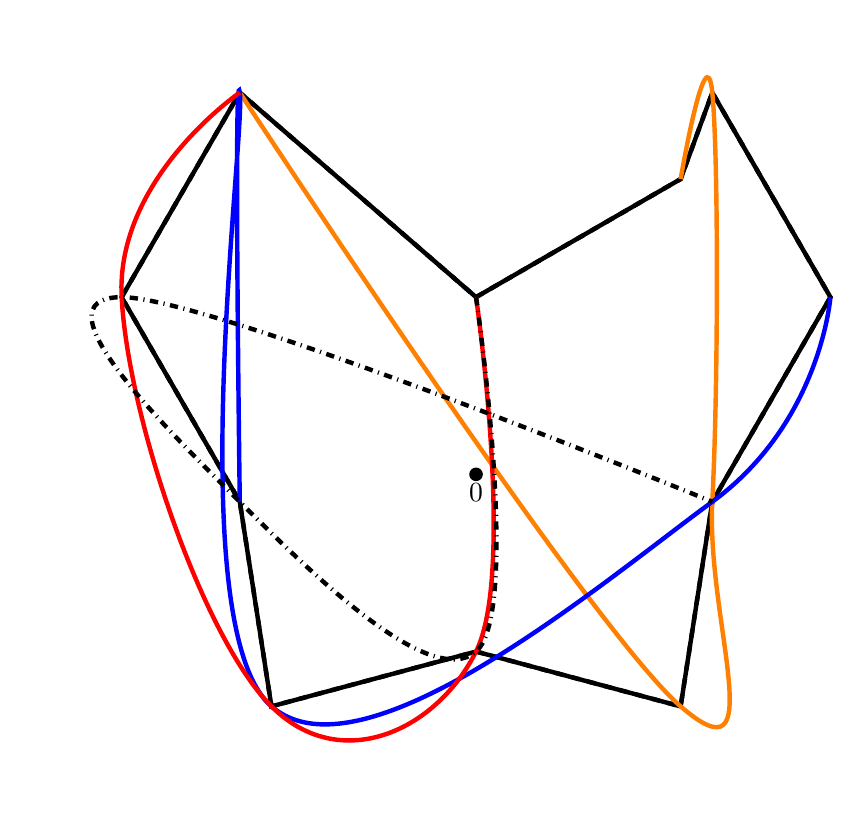
\begin{tikzpicture}[scale=1.5]
        % Define coordinates for the convex hull
        \coordinate (A) at (0,0);
        \coordinate (B) at ({sqrt(3)},1);
        \coordinate (C) at (2,{sqrt(3)});
        \coordinate (D) at (3,0);
        \coordinate (E) at (2,-{sqrt(3)});
        \coordinate (F) at ({sqrt(3)},-{2*sqrt(3)});
        \coordinate (G) at (0,-3);
        \coordinate (H) at (-{sqrt(3)},-{2*sqrt(3)});
        \coordinate (I) at (-2,-{sqrt(3)});
        \coordinate (J) at (-3,0);
        \coordinate (K) at (-2,{sqrt(3)});
        
        % Draw the convex hull and its reflection
        \draw[ultra thick] (A) -- (B) -- (C) -- (D) -- (E) -- (F) -- (G) -- (H) -- (I) -- (J) -- (K) -- cycle;
        \draw[dashed, ultra thick] (A) -- (B) -- (C) -- (D) -- (E) -- (F) -- (G) -- (H) -- (I) -- (J) -- (K) -- cycle;
        
        % Define the Minkowski sum boundaries
        \draw[orange, ultra thick] plot [smooth, tension=0.7] coordinates {(B) (C) (E) (F) (K)};
        \draw[blue, ultra thick] plot [smooth, tension=0.7] coordinates {(D) (E) (H) (K) (I)};
        \draw[red, ultra thick] plot [smooth, tension=0.7] coordinates {(A) (G) (H) (J) (K)};
        \draw[dashdotted, ultra thick] plot [smooth, tension=0.7] coordinates {(A) (G) (I) (J) (E)};
        
        % Mark the origin
        \filldraw (0,-1.5) circle (1.5pt) node[anchor=north] {$0$};
    \end{tikzpicture}
    \caption{}
    \label{fig:example_lemma}
\end{figure}

The common boundary points of $K$ and $-K$ are not boundary points of $\underline{M}_{0}(K,-K)$. Furthermore, the vertices of $\overline{M}_{1}(K,-K)$ are smooth boundary points of $\overline{M}_{\infty}(K,-K)$. By Lemma~\ref{common boundary points lemma}~(ii), $\overline{M}_{p}(K,-K)$ for $p > 1$ is supported at each of these points by exactly one respective line that also supports $K$ and $-K$. However, this does not mean that these points must belong to $K$ or $-K$.

\end{document}